\section{Introduction}% (1 page}


% What is the problem that this project is going to address?
Access management for web applications is a critical component for web
applications.
% Does it matter: why is the problem important?
Many web frameworks provide DSLs to specify security policies for APIs, but
developers still mix the access control of the data with other application
logic.
% Who will benefit when the problem is solved
Although many applications provide official documents for developers,
permission control is often not specific or even missing.
%
Therefore, the goal of this project is to extract a relatively comprehensive
list of security policies for developers to reason about.

We separate the whole project to 4 parts below.
\begin{enumerate}
  \item Identify security-sensitive events. We consider all operations that may
        affect the integrity of database to be security-sensitive events
        (queries that insert, delete, or update the database).

  \item Construct calling-context topology. For each security-sensitive event e,
        builds a topo graph of contexts who start from e and end at program
        entry points.

  \item Generate security policies. For each API,  get the call-chain paths for
        all function calls involve security-sensitive events

  \item Detect Potential Vulnerabilities. Through the policies automatically
        generated by the program, the existing security risks are manually
        identified
\end{enumerate}

From the prior work, We have used doop to taint analysis the lancie api, and got
the corresponding analysis file (such as CallGraphEdge.csv).

Although we have obtained this result, doop itself has compatibility problems
(not compatible with Mac OS), which we cannot solve.

In this project we are using lancie api~\footnote{Publicly available at:
  https://github.com/AreaFiftyLAN/lancie-api.} for analysis use case.
%
Through the analysis of lancie api, we design a simple modeling language below
that describes security policies.
\begin{itemize}
  \item Policy $\rightarrow$ Statement
  \item Principal $\rightarrow$ (Role $|$ Role(Condition) $|$ IsAuthenticated)
        \begin{itemize}
          \item[*] Role $\rightarrow$ ROLE\_ADMIN $|$ ROLE\_OPERATOR $|$ ROLE\_COMMITTEE $|$ ROLE\_USER
          \item[*] Condition $\rightarrow$ string$*$
        \end{itemize}
  \item Action $\rightarrow$ string$*$
  \item Resource $\rightarrow$ string$*$
\end{itemize}

We have written a program that scans the lancie api project file, identifies
security-sensitive events, and automatically generates corresponding
policies (Figure \ref{fig:policies}) based on these Identify security-sensitive
events and call graph. Then we detected Potential Vulnerabilities based on these
policies.
\begin{figure}[htp]
  \centering
  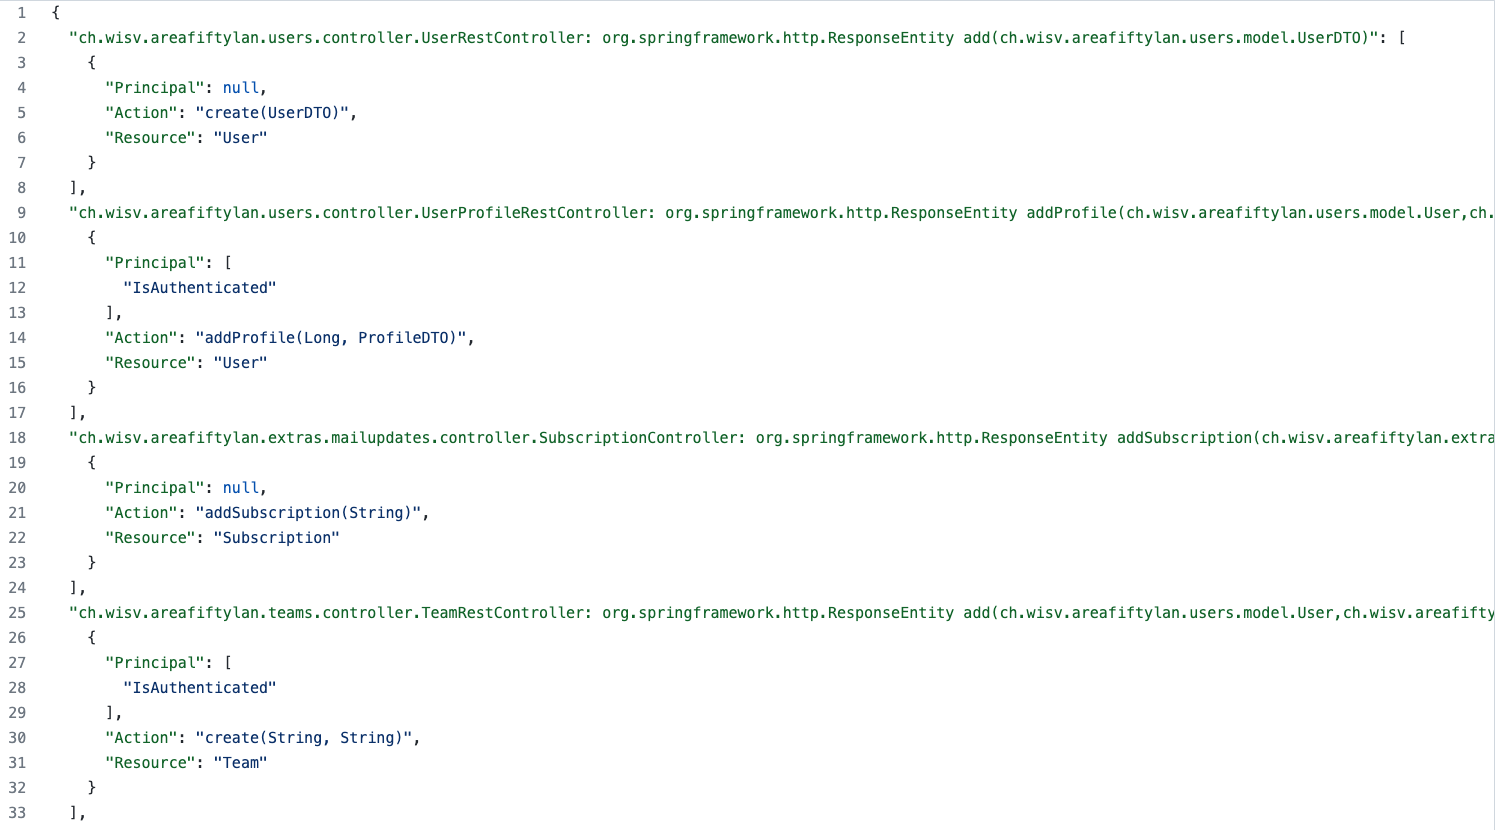
\includegraphics[width=0.45\textwidth]{img/policies.png}
  \caption{polices}
  \label{fig:policies}
\end{figure}

